\newpage
\section{Ôn tập Chương 2}
\def\thoigian{90}%--Thời gian
\de{Đề số 1}{Chương II. Bất phương trình và hệ bất phương trình bậc nhất hai ẩn}

\begin{center}
	\textbf{PHẦN 1 - CÂU TRẮC NGHIỆM BỐN PHƯƠNG ÁN}
\end{center}
\Opensolutionfile{ans}[ans/ans-TN-ONTAPCHUONG-DE1]
%Câu 1
\begin{ex}%[0D2N1-1]%[Dự án D - đợt 2 NH24-25 - VU Ngoc Hao]
	Bất phương trình $3x-2(y-x+1)>0$ tương đương với bất phương trình nào sau đây?
	\choice
	{$x-2y-2>0$}
	{\True $5x-2y-2>0$}
	{$5x-2y-1>0$}
	{$4x-2y-2>0$}
	\loigiai{
	Ta có $3x-2(y-x+1)>0\Leftrightarrow 3x-2y+2x-2>0\Leftrightarrow 5x-2y-2>0$.
	}
\end{ex}
%Câu 2
\begin{ex}%[0D2N1-1]%[Dự án D - đợt 2 NH24-25 - VU Ngoc Hao]
	Cho bất phương trình $x+3+2(2y+5)<2(1-x)$. Khẳng định nào dưới đây là khẳng định \textbf{sai}?
	\choice
	{Điểm $A(-3;-4)$ thuộc miền nghiệm của bất phương trình đã cho}
	{Điểm $B(-2;-5)$ thuộc miền nghiệm của bất phương trình đã cho}
	{Điểm $C(-1;-6)$ thuộc miền nghiệm của bất phương trình đã cho}
	{\True Điểm $O(0;0)$ thuộc miền nghiệm của bất phương trình đã cho}
	\loigiai{
	Lần lượt thay toạ độ điểm ở mỗi phương án vào bất phương trình đã cho, ta thấy\\ $(x_0;y_0)=(0;0)$ không là nghiệm của bất phương trình đã cho.
	}
\end{ex}
%Câu 3
\begin{ex}%[0D2N1-2]%[Dự án D - đợt 2 NH24-25 - VU Ngoc Hao]
	\immini{Hãy chọn bất phương trình mà miền nghiệm của nó là nửa mặt phẳng không bị gạch có bờ là đường thẳng $d$ như hình bên.
	\choicew{0.4\textwidth}
		\choice
		{$x-y>4$}
		{$x-y<4$}
		{$x-y\le 4$}
		{\True $x-y\ge 4$}
	}
	{
		\begin{tikzpicture}[font=\footnotesize, line join=round, line cap=round, >=stealth,scale=0.6]
			\def\xmin{-2} \def\xmax{5}
			\def\ymin{-5} \def\ymax{2}
			\clip(\xmin,\ymin) rectangle (\xmax,\ymax);
			\tkzDefPoints{\xmax/\ymax/A1,\xmin/\ymax/A2,\xmin/\ymin/A3,\xmax/\ymin/A4}
			\tkzDefPoints{5/1/M,-1/-5/N, 4/0/A,0/-4/B}
			\fill[pattern=north east lines,pattern color=black] (M)--(A1)--(A2)--(A3)--(N)--cycle;
			\tkzDrawPoints(A,B)
			\draw[domain=-2:5] plot(\x,{(\x)-4});
			\begin{scriptsize}
				\draw[->](\xmin,0)--(\xmax,0); \draw(\xmax-0.1,0) node[below]{$x$};
				\draw[->](0,\ymin)--(0,\ymax); \draw(0,\ymax-0.2) node[right]{$y$};
				\draw node [above right]{$O$}
				(A) node [below]{$4$}
				(B) node [right]{$-4$}
				(2,-2) node [below]{$d$};
			\end{scriptsize}		
		\end{tikzpicture}
	}
	\loigiai{
	}
\end{ex}
\begin{ex}%[0D2N2-2]%[Lớp 10 - Ôn tập giữa học kì 1 - Chuyên Lên Quý Đôn - Ninh Thuận]%[VU Ngoc Hao]
	\immini{Phần không tô đậm trong hình vẽ dưới đây (không tính bờ) biểu diễn miền nghiệm của hệ bất phương trình nào trong các hệ bất phương trình dưới đây?
	}{\begin{tikzpicture}[>=stealth,line join=round, line cap=round, scale=0.7]
			\draw[->] (-2,0)--(3,0) node[above left]{$x$};
			\draw[->] (0,-3)--(0,3) node[below right]{$y$};
			\clip (-2,-3) rectangle (3,3);
			\fill[pattern=north east 
			lines]plot[domain=-2:3](\x,{(\x)})--plot[domain=3:-2](\x,{3})--cycle;
			\draw[samples=200,smooth,red,line width=1] plot[domain=-2:3]
			(\x,{(\x)});
			\fill[pattern=north east 
			lines]plot[domain=-2:2](\x,{2*(\x)-1})--plot[domain=2:-2](\x,{3})--cycle;
			\draw[samples=200,smooth,red,line width=1] plot[domain=-1:2]
			(\x,{2*(\x)-1}) node[above]{$ $};
			\foreach \x in {1} \draw[fill] (\x,0) circle (1.5pt) 
			node[below]{$\x$};
			\foreach \y in {-1,1} \draw[fill] (0,\y) circle (1.5pt) 
			node[left]{$\y$};
			\draw[dashed] (1,0)--(1,1)--(0,1);
			\fill (0,0) circle (1.5pt) node[above left]{$O$};		\end{tikzpicture}}
	\choice
	{\True $\heva{&x-y>0 \\&2 x-y>1}$}
	{$\heva{&x-y\geq 0 \\&2 x-y \geq 1}$}
	{$\heva{&x-y<0\\&2 x-y>1}$}
	{$\heva{&x-y<0\\&2 x-y<1}$}
	\loigiai{ Gọi $d$ là đường thẳng đi qua hai điểm $O(0;0)$ và $(1;1)$. Suy ra phương trình đường thẳng $d\colon x-y=0$.\\
		Ta thấy điểm $(1;0)$ thuộc miền nghiệm. Thay $x=1$, $y=0$ ta có $1-0>0$. Suy ra bất phương trình thứ nhất là $x-y>0$.\\
		Gọi $d'$ là đường thẳng đi qua hai điểm $(0;-1)$ và $(1;1)$. Suy ra phương trình đường thẳng $d'\colon 2x-y=1$.\\
		Ta thấy điểm $(1;0)$ thuộc miền nghiệm. Thay $x=1$, $y=0$ ta có $2\cdot 1-0>1$. Suy ra bất phương trình thứ hai là $2x-y>1$.\\
		Vậy hệ bất phương trình là $\heva{&x-y>0 \\&2 x-y>1}$.
	}
\end{ex}
%Câu 4
\begin{ex}%[0D2N1-2]%[Dự án D - đợt 2 NH24-25 - VU Ngoc Hao]
	Miền nghiệm của bất phương trình $x+y \leq 2$ là phần không bị gạch sọc của hình vẽ nào trong các hình sau?
	\choice
	{
		\begin{tikzpicture}[scale=1, font=\footnotesize, line join=round, line cap=round, >=stealth]
			\def\xmin{-1}\def\xmax{3.0}\def\ymin{-1}\def\ymax{3.0}
			\draw[->] (\xmin-0.2,0)--(\xmax+0.2,0) node[below] {\footnotesize $x$};
			\draw[->] (0,\ymin-0.2)--(0,\ymax+0.2) node[right] {$y$};
			\draw (0,0) node [below left] {$O$};
			\foreach \x in {-1,1,2,3}\draw (\x,0.1)--(\x,-0.1) node [below] {\footnotesize $\x$};
			\foreach \y in {-1,1,2,3}\draw (0.1,\y)--(-0.1,\y) node [left] {\footnotesize $\y$};
			\clip (\xmin,\ymin) rectangle (\xmax,\ymax);
			\draw[pattern = north west lines,smooth,samples=200,domain=\xmin:\xmax] plot (\x,{-1*(\x)+2});
			\draw[pattern = north east lines,opacity=.3, line width = 1.2pt,draw=none] plot[domain=\xmin:\xmax] (\x, {-1*(\x)+2})--(-1,-1)--(-1,3)--cycle;
		\end{tikzpicture}
	}
	{
		\begin{tikzpicture}[scale=1, font=\footnotesize, line join=round, line cap=round, >=stealth]
			\def\xmin{-3.0}\def\xmax{1}\def\ymin{-1}\def\ymax{3.0}
			\draw[->] (\xmin-0.2,0)--(\xmax+0.2,0) node[below] {\footnotesize $x$};
			\draw[->] (0,\ymin-0.2)--(0,\ymax+0.2) node[right] {$y$};
			\draw (0,0) node [below left] {$O$};
			\foreach \x in {-3,-2,-1,1}\draw (\x,0.1)--(\x,-0.1) node [below] {\footnotesize $\x$};
			\foreach \y in {-1,1,2,3}\draw (0.1,\y)--(-0.1,\y) node [left] {\footnotesize $\y$};
			\clip (\xmin,\ymin) rectangle (\xmax,\ymax);
			\draw[pattern = north west lines,smooth,samples=200,domain=\xmin:\xmax] plot (\x,{1*(\x)+2});
			\draw[pattern = north east lines,opacity=.3, line width = 1.2pt,draw=none] plot[domain=\xmin:\xmax] (\x, {1*(\x)+2})--(1,3)--(1,-1)--cycle;
		\end{tikzpicture}
	}
	{\True
		\begin{tikzpicture}[scale=1, font=\footnotesize, line join=round, line cap=round, >=stealth]
			\def\xmin{-1}\def\xmax{3.0}\def\ymin{-1}\def\ymax{3.0}
			\draw[->] (\xmin-0.2,0)--(\xmax+0.2,0) node[below] {\footnotesize $x$};
			\draw[->] (0,\ymin-0.2)--(0,\ymax+0.2) node[right] {$y$};
			\draw (0,0) node [below left] {$O$};
			\foreach \x in {-1,1,2,3}\draw (\x,0.1)--(\x,-0.1) node [below] {\footnotesize $\x$};
			\foreach \y in {-1,1,2,3}\draw (0.1,\y)--(-0.1,\y) node [left] {\footnotesize $\y$};
			\clip (\xmin,\ymin) rectangle (\xmax,\ymax);
			\draw[pattern = north west lines,smooth,samples=200,domain=\xmin:\xmax] plot (\x,{-1*(\x)+2});
			\draw[pattern = north east lines,opacity=.3, line width = 1.2pt,draw=none] plot[domain=\xmin:\xmax] (\x, {-1*(\x)+2})--(3,3)--(-1,3)--cycle;
		\end{tikzpicture}
	}
	{
		\begin{tikzpicture}[scale=1, font=\footnotesize, line join=round, line cap=round, >=stealth]
			\def\xmin{-3.0}\def\xmax{1}\def\ymin{-1}\def\ymax{3.0}
			\draw[->] (\xmin-0.2,0)--(\xmax+0.2,0) node[below] {\footnotesize $x$};
			\draw[->] (0,\ymin-0.2)--(0,\ymax+0.2) node[right] {$y$};
			\draw (0,0) node [below left] {$O$};
			\foreach \x in {-3,-2,-1,1}\draw (\x,0.1)--(\x,-0.1) node [below] {\footnotesize $\x$};
			\foreach \y in {-1,1,2,3}\draw (0.1,\y)--(-0.1,\y) node [left] {\footnotesize $\y$};
			\clip (\xmin,\ymin) rectangle (\xmax,\ymax);
			\draw[pattern = north west lines,smooth,samples=200,domain=\xmin:\xmax] plot (\x,{1*(\x)+2});
			\draw[pattern = north east lines,opacity=.3, line width = 1.2pt,draw=none] plot[domain=\xmin:\xmax] (\x, {1*(\x)+2})--(-3,3)--(-3,-1)--cycle;
		\end{tikzpicture}
	}
	\loigiai{
		\immini{
			Biểu diễn miền nghiệm trên mặt phẳng $Oxy$:\\
			- Vẽ đường thẳng $d: x+y=2$.\\
			- Lấy điểm $O(0;0)$ thay tọa độ vào ta có $0+0 \leq 2$ đúng.\\
			Vậy miền nghiệm bất phương trình là nửa mặt phẳng chứa điểm $O(0;0)$ và có bờ là đường thẳng $d$, kể cả đường thẳng $d$.
		}{
			\begin{tikzpicture}[scale=1, font=\footnotesize, line join=round, line cap=round, >=stealth]
				\def\xmin{-1}\def\xmax{3.0}\def\ymin{-1}\def\ymax{3.0}
				\draw[->] (\xmin-0.2,0)--(\xmax+0.2,0) node[below] {\footnotesize $x$};
				\draw[->] (0,\ymin-0.2)--(0,\ymax+0.2) node[right] {$y$};
				\draw (0,0) node [below left] {$O$};
				\foreach \x in {-1,1,2,3}\draw (\x,0.1)--(\x,-0.1) node [below] {\footnotesize $\x$};
				\foreach \y in {-1,1,2,3}\draw (0.1,\y)--(-0.1,\y) node [left] {\footnotesize $\y$};
				\clip (\xmin,\ymin) rectangle (\xmax,\ymax);
				\draw[pattern = north west lines,smooth,samples=200,domain=\xmin:\xmax] plot (\x,{-1*(\x)+2});
				\draw[pattern = north east lines,opacity=.3, line width = 1.2pt,draw=none] plot[domain=\xmin:\xmax] (\x, {-1*(\x)+2})--(3,3)--(-1,3)--cycle;
			\end{tikzpicture}
		}
	}
\end{ex}
%Câu 5
\begin{ex}%[0D2H1-3]%[Dự án D - đợt 2 NH24-25 - VU Ngoc Hao]
	Một người thợ mộc tốn $6$ giờ để làm một cái bàn và $4$ giờ để làm một cái ghế. Gọi $x$, $y$ lần lượt là số bàn và số ghế mà người thợ mộc sản xuất trong một tuần. Viết bất phương trình biểu thị mối liên hệ giữa $x$ và $y$ biết trong một tuần người thợ mộc có thể làm tối đa $50$ giờ.
	\choice
	{\True $3x+2y\le 25$}
	{$3x+2y> 25$}
	{$3x+2y\ge 25$}
	{$3x+2y< 25$}
	\loigiai{
	Trong một tuần, số giờ làm ra $x$ cái bàn là $6x$ và số giờ làm ra $y$ cái ghế là $4y$.\\
		Vì trong một tuần người thợ mộc làm tối đa $50$ giờ nên 
		$$6x+4y\le 50\Leftrightarrow 3x+2y\le 25.$$
	}
\end{ex}
%Câu 6
\begin{ex}%[0D2V1-3]%[Dự án D - đợt 2 NH24-25 - VU Ngoc Hao]
	Một gia đình cần $x$ kg thịt bò và $y$ kg thịt lợn trong một ngày, giá tiền $1$ kg thịt bò là $200$ nghìn đồng, $1$ kg thịt lợn là $60$ nghìn đồng. Trong các phần hình phẳng không bị gacgh cho sau đây, phần hình phẳng nào mô tả chi phí gia đình đó mua thịt bò và thịt lợn mỗi ngày để số tiền bỏ ra trong một ngày không quá $300$ nghìn đồng?
	\choice
	{\True \begin{tikzpicture}[scale=.7,font=\footnotesize, line join=round, line cap=round, >=stealth]
			\tikzset{label style/.style={font=\footnotesize}}
			\begin{scope}
				\clip (0,0) rectangle (4,6);
				\fill[pattern=north east lines] (-1,8.33)--(5,8.33)--(5,-11.67)--cycle;
				\draw (-0.3,6)--(1.5,0) node [pos=0.45, above, sloped] {};
			\end{scope}
			\draw[->] (0,0)--(4,0) node[below]{$x$};
			\draw[->] (0,0)--(0,6) node[left]{$y$};
			\draw (0,0) node[below left]{$O$};
			\draw (1.5,0) node[below]{$1{,}5$};
			\foreach \y in {5}
			\draw[thin] (1pt,\y)--(-1pt,\y) node [left] {$\y$};
	\end{tikzpicture}}
	{\begin{tikzpicture}[scale=.7,font=\footnotesize, line join=round, line cap=round, >=stealth]
			\tikzset{label style/.style={font=\footnotesize}}
			\begin{scope}
				\clip (0,0) rectangle (4,6);
				\fill[pattern=north east lines] (-1,8.33)--(-1,-11.67)--(5,-11.67)--cycle;
				\draw (-0.3,6)--(1.5,0) node [pos=0.45, above, sloped] {};
			\end{scope}
			\draw[->] (0,0)--(4,0) node[below]{$x$};
			\draw[->] (0,0)--(0,6) node[left]{$y$};
			\draw (0,0) node[below left]{$O$};
			\draw (1.5,0) node[below]{$1{,}5$};
			\foreach \y in {5}
			\draw[thin] (1pt,\y)--(-1pt,\y) node [left] {$\y$};
	\end{tikzpicture}}
	{\begin{tikzpicture}[scale=.7,font=\footnotesize, line join=round, line cap=round, >=stealth]
			\tikzset{label style/.style={font=\footnotesize}}
			\begin{scope}
				\clip (0,0) rectangle (4,6);
				\fill[pattern=north east lines] (-1,8.33)--(5,8.33)--(5,-11.67)--cycle;
				\draw (-0.3,6)--(1.5,0) node [pos=0.45, above, sloped] {};
			\end{scope}
			\draw[->] (0,0)--(4,0) node[below]{$x$};
			\draw[->] (0,0)--(0,6) node[left]{$y$};
			\draw (0,0) node[below left]{$O$};
			\draw (1.5,0) node[below]{$1$};
			\foreach \y in {5}
			\draw[thin] (1pt,\y)--(-1pt,\y) node [left] {$\y$};
	\end{tikzpicture}}
	{\begin{tikzpicture}[scale=.7,font=\footnotesize, line join=round, line cap=round, >=stealth]
			\tikzset{label style/.style={font=\footnotesize}}
			\begin{scope}
				\clip (0,0) rectangle (4,6);
				\fill[pattern=north east lines] (-1,8.33)--(-1,-11.67)--(5,-11.67)--cycle;
				\draw (-0.3,6)--(1.5,0) node [pos=0.45, above, sloped] {};
			\end{scope}
			\draw[->] (0,0)--(4,0) node[below]{$x$};
			\draw[->] (0,0)--(0,6) node[left]{$y$};
			\draw (0,0) node[below left]{$O$};
			\draw (1.5,0) node[below]{$1$};
			\foreach \y in {5}
			\draw[thin] (1pt,\y)--(-1pt,\y) node [left] {$\y$};
	\end{tikzpicture}}
	\loigiai{
		Số tiền mua thịt bò là $200x$ và số tiền mua thịt lợn là $60y$.\\
		Tổng số tiền trong một ngày mua thịt lợn và thịt bò là $200x+60y$.\\
		Để chi phí mua thịt bò và thịt lợn mỗi ngày không quá $300$ nghìn đồng thì 
		$$200x+60y\le 300\Leftrightarrow 10x+3y\le 15.$$
		Khi đó, phần hình phẳng cần tìm là 
		\begin{center}
			\begin{tikzpicture}[scale=.7,font=\footnotesize, line join=round, line cap=round, >=stealth]
				\tikzset{label style/.style={font=\footnotesize}}
				\begin{scope}
					\clip (0,0) rectangle (4,6);
					\fill[pattern=north east lines] (-1,8.33)--(5,8.33)--(5,-11.67)--cycle;
					\draw (-0.3,6)--(1.5,0) node [pos=0.45, above, sloped] {};
				\end{scope}
				\draw[->] (0,0)--(4,0) node[below]{$x$};
				\draw[->] (0,0)--(0,6) node[left]{$y$};
				\draw (0,0) node[below left]{$O$};
				\draw (1.5,0) node[below]{$1{,}5$};
				\foreach \y in {5}
				\draw[thin] (1pt,\y)--(-1pt,\y) node [left] {$\y$};
			\end{tikzpicture}
		\end{center}
	}
\end{ex}
%Câu 7
\begin{ex}%[0D2N2-1]%[Dự án D - đợt 2 NH24-25 - VU Ngoc Hao]
	Cho hệ bất phương trình $\heva{& x+3y-2\geq 0\\ & 2x+y+1\leq 0}$. Trong các điểm sau, điểm nào thuộc miền nghiệm của hệ bất phương trình?
	\choice
	{$M\left(0;1\right)$}
	{\True $N\left(-1;1\right)$}
	{$P\left(1;3\right)$}
	{$Q\left(-1;0\right)$}
	\loigiai{
	Thay toạ độ điểm $N\left(-1;1\right)$ vào hệ bất phương trình ta có $\heva{& -1+3-2\geq 0\\ & -2+1+1\leq 0}$ (đúng). Do đó, điểm $N$ thuộc miền nghiệm của hệ bất phương trình.	
	}
\end{ex}


%Câu 8
\begin{ex}%[0D2N2-1]%[Dự án D - đợt 2 NH24-25 - VU Ngoc Hao]
	Cho hệ bất phương trình $\heva{& 2x-5y-1>0\\ & 2x+y+5>0 \\& x+y+1<0}$. Trong các điểm sau, điểm nào thuộc miền nghiệm của hệ bất phương trình?
	\choice
	{$O\left(0;0\right)$}
	{$M\left(1;0\right)$}
	{\True $N\left(0;-2\right)$}
	{$P\left(0;2\right)$}
	\loigiai{
		Thay toạ độ điểm $N\left(0;-2\right)$ vào hệ bất phương trình ta có $\heva{& 10-1> 0\\ & -2+5> 0\\ & -2+1<0}$ (đúng). Do đó, điểm $N$ thuộc miền nghiệm của hệ bất phương trình.		
	}
	
\end{ex}
%Câu 9
\begin{ex}%[0D2N2-1]%[Dự án D - đợt 2 NH24-25 - VU Ngoc Hao]
	Cho hệ bất phương trình $\heva{& x+y-2\leq 0\\ & 2x-3y+2>0}$. Trong các điểm sau, điểm nào \textbf{không thuộc} miền nghiệm của hệ bất phương trình?
	\choice
	{$O\left(0;0\right)$}
	{$M\left(1;1\right)$}
	{\True $N\left(-1;1\right)$}
	{$P\left(-1;-1\right)$}
	\loigiai{
		Thay toạ độ điểm $N\left(-1;1\right)$ vào hệ bất phương trình ta có: $\heva{& -1+1-2\leq 0\\ & -2-3+2> 0}$ (vô lý). Do đó, điểm $N$ không thuộc miền nghiệm của hệ bất phương trình.		
	}
	
\end{ex}

%Câu 10

\begin{ex}%[0D2H2-2]%[Dự án D - đợt 2 NH24-25 - VU Ngoc Hao]
	Miền nghiệm của hệ bất phương trình $\heva{& x-2y<0\\ & x+3y>-2\\ & y-x<3}$ là phần không tô đậm của hình vẽ nào trong các hình vẽ sau?
	\choice
	{\True \begin{tikzpicture}[line join=round, line cap=round, >=stealth,font=\footnotesize, scale=0.4]
			% Vẽ hệ trục toạ độ
			\draw (0,0) node [right] {$O$};
			\draw [->] (-6.5,0)--(4.5,0) node[below]{$x$};
			\draw[->] (0,-6.5)--(0,4.5) node[left]{$y$};
			\clip(-6.5,-6.5) rectangle (4.5,4.5);
			% Vẽ các số trên hai trục
			\foreach \x in {-3,-2}
			\draw[shift={(\x,0)},color=black] (0pt,2pt) -- (0pt,-2pt) node[below] {\footnotesize $\x$};
			\foreach \y in {3}
			\draw[shift={(0,\y)},color=black] (2pt,0pt) -- (-2pt,0pt)node[right] {\footnotesize $\y$};
			%Vẽ đồ thị từng hàm số
			\draw[samples=100,smooth,domain=-6.5:4.5,black] plot(\x,{0.5*(\x)});
			\draw[samples=100,smooth,domain=-6.5:4.5,black] plot(\x,{-0.33333333*(\x)-0.6666666666});
			\draw[samples=100,smooth,domain=-6.5:4.5,black] plot(\x,{(\x)+3});
			% Vẽ miền nghiệm
			\fill[pattern=north west lines,opacity=0.6] plot[domain=-6.5:4.5](\x,{(\x)+3})--plot[domain=4.5:-6.5](\x,{4.5})--cycle;
			\fill[pattern=north west lines,opacity=0.6] plot[domain=-6.5:4.5](\x,{-0.33333333*(\x)-0.6666666666})--plot[domain=4.5:-6.5](\x,{-6.5})--cycle;
			\fill[pattern=north west lines,opacity=0.6] plot[domain=-6.5:4.5](\x,{0.5*(\x)})--plot[domain=4.5:-6.5](\x,{-6.5})--cycle;
	\end{tikzpicture}}
	{\begin{tikzpicture}[line join=round, line cap=round, >=stealth,font=\footnotesize, scale=0.4]
			% Vẽ hệ trục toạ độ
			\draw (0,0) node [right] {$O$};
			\draw [->] (-6.5,0)--(4.5,0) node[below]{$x$};
			\draw[->] (0,-6.5)--(0,4.5) node[left]{$y$};
			\clip(-6.5,-6.5) rectangle (4.5,4.5);
			% Vẽ các số trên hai trục
			\foreach \x in {-3,-2}
			\draw[shift={(\x,0)},color=black] (0pt,2pt) -- (0pt,-2pt) node[below] {\footnotesize $\x$};
			\foreach \y in {3}
			\draw[shift={(0,\y)},color=black] (2pt,0pt) -- (-2pt,0pt)node[right] {\footnotesize $\y$};
			%Vẽ đồ thị từng hàm số
			\draw[samples=100,smooth,domain=-6.5:4.5,black] plot(\x,{0.5*(\x)});
			\draw[samples=100,smooth,domain=-6.5:4.5,black] plot(\x,{-0.33333333*(\x)-0.6666666666});
			\draw[samples=100,smooth,domain=-6.5:4.5,black] plot(\x,{(\x)+3});
			% Vẽ miền nghiệm
			\fill[pattern=north west lines,opacity=0.6] plot[domain=-6.5:4.5](\x,{(\x)+3})--plot[domain=4.5:-6.5](\x,{4.5})--cycle;
			\fill[pattern=north west lines,opacity=0.6] plot[domain=-6.5:4.5](\x,{-0.33333333*(\x)-0.6666666666})--plot[domain=4.5:-6.5](\x,{4.5})--cycle;
			\fill[pattern=north west lines,opacity=0.6] plot[domain=-6.5:4.5](\x,{0.5*(\x)})--plot[domain=4.5:-6.5](\x,{-6.5})--cycle;
	\end{tikzpicture}}
	{\begin{tikzpicture}[line join=round, line cap=round, >=stealth,font=\footnotesize, scale=0.4]
			% Vẽ hệ trục toạ độ
			\draw (0,0) node [right] {$O$};
			\draw [->] (-6.5,0)--(4.5,0) node[below]{$x$};
			\draw[->] (0,-6.5)--(0,4.5) node[left]{$y$};
			\clip(-6.5,-6.5) rectangle (4.5,4.5);
			% Vẽ các số trên hai trục
			\foreach \x in {-3,-2}
			\draw[shift={(\x,0)},color=black] (0pt,2pt) -- (0pt,-2pt) node[below] {\footnotesize $\x$};
			\foreach \y in {3}
			\draw[shift={(0,\y)},color=black] (2pt,0pt) -- (-2pt,0pt)node[right] {\footnotesize $\y$};
			%Vẽ đồ thị từng hàm số
			\draw[samples=100,smooth,domain=-6.5:4.5,black] plot(\x,{0.5*(\x)});
			\draw[samples=100,smooth,domain=-6.5:4.5,black] plot(\x,{-0.33333333*(\x)-0.6666666666});
			\draw[samples=100,smooth,domain=-6.5:4.5,black] plot(\x,{(\x)+3});
			% Vẽ miền nghiệm
			\fill[pattern=north west lines,opacity=0.6] plot[domain=-6.5:4.5](\x,{(\x)+3})--plot[domain=4.5:-6.5](\x,{4.5})--cycle;
			\fill[pattern=north west lines,opacity=0.6] plot[domain=-6.5:4.5](\x,{-0.33333333*(\x)-0.6666666666})--plot[domain=4.5:-6.5](\x,{4.5})--cycle;
			\fill[pattern=north west lines,opacity=0.6] plot[domain=-6.5:4.5](\x,{0.5*(\x)})--plot[domain=4.5:-6.5](\x,{4.5})--cycle;
	\end{tikzpicture}}
	{\begin{tikzpicture}[line join=round, line cap=round, >=stealth,font=\footnotesize, scale=0.4]
			% Vẽ hệ trục toạ độ
			\draw (0,0) node [right] {$O$};
			\draw [->] (-6.5,0)--(4.5,0) node[below]{$x$};
			\draw[->] (0,-6.5)--(0,4.5) node[left]{$y$};
			\clip(-6.5,-6.5) rectangle (4.5,4.5);
			% Vẽ các số trên hai trục
			\foreach \x in {-3,-2}
			\draw[shift={(\x,0)},color=black] (0pt,2pt) -- (0pt,-2pt) node[below] {\footnotesize $\x$};
			\foreach \y in {3}
			\draw[shift={(0,\y)},color=black] (2pt,0pt) -- (-2pt,0pt)node[right] {\footnotesize $\y$};
			%Vẽ đồ thị từng hàm số
			\draw[samples=100,smooth,domain=-6.5:4.5,black] plot(\x,{0.5*(\x)});
			\draw[samples=100,smooth,domain=-6.5:4.5,black] plot(\x,{-0.33333333*(\x)-0.6666666666});
			\draw[samples=100,smooth,domain=-6.5:4.5,black] plot(\x,{(\x)+3});
			% Vẽ miền nghiệm
			\fill[pattern=north west lines,opacity=0.6] plot[domain=-6.5:4.5](\x,{(\x)+3})--plot[domain=4.5:-6.5](\x,{-6.5})--cycle;
			\fill[pattern=north west lines,opacity=0.6] plot[domain=-6.5:4.5](\x,{-0.33333333*(\x)-0.6666666666})--plot[domain=4.5:-6.5](\x,{4.5})--cycle;
			\fill[pattern=north west lines,opacity=0.6] plot[domain=-6.5:4.5](\x,{0.5*(\x)})--plot[domain=4.5:-6.5](\x,{-6.5})--cycle;
	\end{tikzpicture}}
	\loigiai{
		Xét đường thẳng $d:  x-2y=0 $.\\
		Thay tọa độ điểm $(-1;0)$ vào vế trái phương trình đường thẳng $(d)$, ta được: $-1<0$.\\
		Vậy miền nghiệm của bất phương trình $x-2y<0$ là nửa mặt phẳng chứa điểm $(-1,0)$, không kể cả bờ $(d)$.\\
		Do chỉ có hình 
		\begin{center}
			\begin{tikzpicture}[line join=round, line cap=round, >=stealth,font=\footnotesize, scale=0.4]
				% Vẽ hệ trục toạ độ
				\draw (0,0) node [right] {$O$};
				\draw [->] (-6.5,0)--(4.5,0) node[below]{$x$};
				\draw[->] (0,-6.5)--(0,4.5) node[left]{$y$};
				\clip(-6.5,-6.5) rectangle (4.5,4.5);
				% Vẽ các số trên hai trục
				\foreach \x in {-3,-2}
				\draw[shift={(\x,0)},color=black] (0pt,2pt) -- (0pt,-2pt) node[below] {\footnotesize $\x$};
				\foreach \y in {3}
				\draw[shift={(0,\y)},color=black] (2pt,0pt) -- (-2pt,0pt)node[right] {\footnotesize $\y$};
				%Vẽ đồ thị từng hàm số
				\draw[samples=100,smooth,domain=-6.5:4.5,black] plot(\x,{0.5*(\x)});
				\draw[samples=100,smooth,domain=-6.5:4.5,black] plot(\x,{-0.33333333*(\x)-0.6666666666});
				\draw[samples=100,smooth,domain=-6.5:4.5,black] plot(\x,{(\x)+3});
				% Vẽ miền nghiệm
				\fill[pattern=north west lines,opacity=0.6] plot[domain=-6.5:4.5](\x,{(\x)+3})--plot[domain=4.5:-6.5](\x,{4.5})--cycle;
				\fill[pattern=north west lines,opacity=0.6] plot[domain=-6.5:4.5](\x,{-0.33333333*(\x)-0.6666666666})--plot[domain=4.5:-6.5](\x,{-6.5})--cycle;
				\fill[pattern=north west lines,opacity=0.6] plot[domain=-6.5:4.5](\x,{0.5*(\x)})--plot[domain=4.5:-6.5](\x,{-6.5})--cycle;
			\end{tikzpicture}
		\end{center}
		chứa điểm $(-1;0)$ nên ta chọn hình này.
	}
	
\end{ex}

%Câu 11
\begin{ex}[Trích đề thi GHKI - Khối 10 - chuyên Lê Quý Đôn Ninh Thuận Năm học 2023 - 2024]%[0D2H2-2]%[Dự án đề kiểm tra Toán 10 GHKI NH23-24- Phạm Hoài]%[THPT Lê Quý Đôn - Ninh Thuận]
	\immini{Tập hợp các điểm $M(x, y)$ thoả mãn hệ bất phương trình $\heva{&x+y \geq 2 \\& x+y \leq 5 \\& x-2 y \leq-1 \\& x-2 y \leq-4}$.\\
		là miền tứ giác như hình bên (phần không bị gạch bỏ trong hình vẽ). Giá trị lớn nhất của biểu thức $F(x;y)=15 x+30 y$ bằng
		\choice
		{$150$ }
		{$105$ }
		{\True $120$ }
		{$135$ }}
	{\begin{tikzpicture}[line join=round, line cap=round, >=stealth,font=\footnotesize, scale=0.8]
			\draw[->](-1,0)--(4,0) node[below] {$x$};
			\draw[->](0,-1)--(0,4) node[right] {$y$};
			\node (0,0) [below right]{$ O $};
			\draw[samples=100,smooth,domain=-1:3,red] plot(\x,{-1*(\x)+2});
			\draw[samples=100,smooth,domain=1:4,red] plot(\x,{-1*(\x)+5});
			\draw[samples=100,smooth,domain=-1:4,red] plot(\x,{0.5*(\x)+2});
			\draw[samples=100,smooth,domain=-1:4,red] plot(\x,{0.5*(\x)+0.5});
			\fill[pattern=north east lines,pattern color=blue] (-1,3)--(-1,-1)-- (3,-1)--cycle;
			\fill[pattern=north east lines,pattern color=blue] (1,4)--(4,4)-- (4,1)--cycle;
			\fill[pattern=north east lines,pattern color=blue] (-1,4)--(-1,1.5)-- (4,4)--cycle;
			\fill[pattern=north east lines,pattern color=blue] (-1,0)--(-1,-1)-- (4,-1)--(4,2.5)--cycle;
			\draw[dashed](1,0)circle(1pt)node[below] {$1$}--(1,1)--(0,1)circle(1pt)node[ left] {$1$};
			\draw[dashed](2,0)circle(1pt)node[below] {$2$}--(2,3)--(0,3)circle(1pt)node[ left] {$3$};
			\draw[dashed](3,0)circle(1pt)node[below] {$3$}--(3,2)--(0,2)circle(1pt)node[ left] {$2$};
	\end{tikzpicture}}
	\loigiai{
		\immini{Miền nghiệm thu được của hệ bất phương trình trên là tứ giác $ABCD$ với các đỉnh lần lượt là $A(0,2)$, $B(1,1)$, $C(3,2)$, $D(2,3)$.\\
			Khi đó\\
			Tại đỉnh $A(2;0)$, ta có $F(2;0)=15 \cdot 0+30\cdot 2=60$.\\
			Tại đỉnh $B(1;1)$, ta có $F(1;1)=15 \cdot 1+30\cdot 1=45$.\\
			Tại đỉnh $C(3;2)$, ta có $F(3;2)=15 \cdot 2+30\cdot 3=120$.\\
			Tại đỉnh $D(2;3)$, ta có $F(2;3)=15 \cdot 3+30\cdot 2=105$.\\
			Vậy giá trị lớn nhất của $F$ là $120$ tại $C(3;2)$.}	
		{\begin{tikzpicture}[line join=round, line cap=round, >=stealth,font=\footnotesize, scale=0.8]
				\draw[->](-1,0)--(4,0) node[below] {$x$};
				\draw[->](0,-1)--(0,4) node[right] {$y$};
				\node (0,0) [below right]{$ O $};
				\draw[samples=100,smooth,domain=-1:3,red] plot(\x,{-1*(\x)+2});
				\draw[samples=100,smooth,domain=1:4,red] plot(\x,{-1*(\x)+5});
				\draw[samples=100,smooth,domain=-1:4,red] plot(\x,{0.5*(\x)+2});
				\draw[samples=100,smooth,domain=-1:4,red] plot(\x,{0.5*(\x)+0.5});
				\fill[pattern=north east lines,pattern color=blue] (-1,3)--(-1,-1)-- (3,-1)--cycle;
				\fill[pattern=north east lines,pattern color=blue] (1,4)--(4,4)-- (4,1)--cycle;
				\fill[pattern=north east lines,pattern color=blue] (-1,4)--(-1,1.5)-- (4,4)--cycle;
				\fill[pattern=north east lines,pattern color=blue] (-1,0)--(-1,-1)-- (4,-1)--(4,2.5)--cycle;
				\draw[dashed](1,0)circle(1pt)node[below] {$1$}--(1,1)--(0,1)circle(1pt)node[ left] {$1$};
				\draw[dashed](2,0)circle(1pt)node[below] {$2$}--(2,3)--(0,3)circle(1pt)node[ left] {$3$};
				\draw[dashed](3,0)circle(1pt)node[below] {$3$}--(3,2)--(0,2)circle(1pt)node[ left] {$2$};
				\draw[dashed](0,2)node[right] {$A$}(1,1)node[ above] {$B$}(3,2)node[left] {$C$}(2,3)node[below] {$D$};
		\end{tikzpicture}}	
	}
\end{ex}
%Câu 12
\begin{ex}%[0D2V2-2]%[Dự án D - đợt 2 NH24-25 - VU Ngoc Hao]
	Biểu thức $F(x;y)=y-x$ đạt giá trị nhỏ nhất với điều kiện $\heva{& 2x-y\geq 2\\ & x-2y\leq 2\\ & x+y\leq 5\\ & x\geq 0}$ tại điểm $M$ có toạ độ là
	\choice
	{\True $\left(4;1\right)$}
	{$\left(\dfrac{8}{3};\dfrac{7}{3}\right)$}
	{$\left(\dfrac{2}{3};-\dfrac{2}{3}\right)$}
	{$\left(5;0\right)$}
	\loigiai{
		Miền nghiệm của hệ bất phương trình là miền đa giác $ABCD$ với  $A(1;0)$, $B\left(\dfrac{7}{3};\dfrac{8}{3}\right)$, $C(4;1)$ và $D(2,0)$
		\begin{center}
			\begin{tikzpicture}[line join=round, line cap=round, >=stealth,font=\footnotesize, scale=0.8]
				% Vẽ hệ trục toạ độ
				\draw (0,0) node [below right] {$O$};
				\draw [->] (-0.5,0)--(5.5,0) node[below]{$x$};
				\draw[->] (0,-2.5)--(0,5.5) node[left]{$y$};
				\clip(-1,-3) rectangle (5.5,5.5);
				% Vẽ các số trên hai trục
				\foreach \x in {1,2,5}
				\draw[shift={(\x,0)},color=black] (0pt,2pt) -- (0pt,-2pt) node[below] {\footnotesize $\x$};
				\foreach \y in {-2,-1,5}
				\draw[shift={(0,\y)},color=black] (2pt,0pt) -- (-2pt,0pt)node[left] {\footnotesize $\y$};
				%Vẽ đồ thị từng hàm số
				\draw[samples=100,smooth,domain=-0.5:5.5,black] plot(\x,{2*(\x)-2});
				\draw[samples=100,smooth,domain=-0.5:5.5,black] plot(\x,{0.5*(\x)-1});
				\draw[samples=100,smooth,domain=-0.5:5.5,black] plot(\x,{5-(\x)});
				% Vẽ miền nghiệm
				\fill[pattern=north east lines,opacity=0.6] plot[domain=-0.5:5.5](\x,{2*(\x)-2})--plot[domain=5.5:-0.5](\x,{5.5})--cycle;
				\fill[pattern=north east lines,opacity=0.6] plot[domain=-0.5:5.5](\x,{0.5*(\x)-1})--plot[domain=5.5:-0.5](\x,{-2.5})--cycle;
				\fill[pattern=north east lines,opacity=0.6] plot[domain=-0.5:5.5](\x,{5-(\x)})--plot[domain=5.5:-0.5](\x,{5.5})--cycle;
				\fill[pattern=north east lines,opacity=0.6] plot[domain=-0.5:5.5](\x,{0})--plot[domain=5.5:-0.5](\x,{-2.5})--cycle;
				\draw (1,0.2) node [above left] {$A$};
				\draw (2.3333,2.9) node [below left] {$B\left(\dfrac{7}{3};\dfrac{8}{3}\right)$};
				\draw (4,1.2) node [above right] {$C$};
				\draw (2,0) node [above right] {$D$};
				\fill (1,0) circle (2pt);
				\fill  (2.3333333, 2.66666666)  circle (2pt);
				\fill (2,0) circle (2pt);
				\fill (4,1) circle (2pt);
			\end{tikzpicture}
		\end{center}
		Ta có: $F(1;0)=-1$, $F\left(\dfrac{7}{3},\dfrac{8}{3}\right)=\dfrac{1}{3}$, $F(4;1)=-3$ và $F(2;0)=-2$. Do đó, $\mathop{\min}F=-3$ khi $x=4$, $y=1$.\\
		Vậy $M(4;1)$.
	}
	
\end{ex}

\Closesolutionfile{ans}
%\begin{center}
%	\textbf{ĐÁP ÁN}
%	\inputansbox{10}{ans/ans}	
%\end{center}

\begin{center}
	\textbf{PHẦN 2 - CÂU TRẮC NGHIỆM ĐÚNG SAI}
\end{center}
\setcounter{ex}{0}
\Opensolutionfile{ans}[ans/answer-DS-ONTAPCHUONG-DE1]
%Câu 1
\begin{ex}[Trích đề thi dự bị CHKI - Khối 10 - chuyên Lê Quý Đôn Ninh Thuận Năm học 2024 - 2025]%[0D2H2-2]%[Dự án D - đợt 2 NH24-25 - VU Ngoc Hao]
	Cho bất phương trình $2x-3y\ge 6\quad (1)$.
	\choiceTF
	{Bất phương trình $(1)$ là bất phương trình bậc hai một ẩn}
	{\True Cặp số $(x;y)=(3;0)$ thuộc miền nghiệm của bất phương trình $(1)$}
	{Miền nghiệm của bất phương trình $(1)$ là miền tô đậm không bao gồm bờ $d$}
	{\True Miền nghiệm của bất phương trình $(1)$ là miền không tô đậm, bao gồm cả bờ $d$}
	\centering{	\begin{tikzpicture}[scale=.9,font=\footnotesize,>=stealth]
			%---------------------- Vẽ hệ trục tọa độ
			\draw[->] (-1,0)--(5,0) node[below right] {$x$};
			\draw[->] (0,-2.7)--(0,1.4) node[above right] {$y$};
			\node (0,0) [below left]{$ O $};
			%----------------------- Vẽ đoạn chắn trên trục
			\foreach \x in {1,2,3,4}
			\draw[shift={(\x,0)},color=black] (0pt,2pt) -- (0pt,-2pt);
			%\node at (3.8,0.5) {$4$};
			\foreach \y in {-2,-1,1}
			\draw[shift={(0,\y)},color=black] (2pt,0pt) -- (-2pt,0pt);
			%\node at (-0.5,-1.8) {$-2$};
			
			%--------------------- Vẽ hàm
			\draw [thick, domain=-1:5, samples=100] plot (\x, {(2/3) * \x-2});
			\node[left] at (2,-1) {$d$};
			\node[right] at (0,-2) {$-2$};
			\node[below] at (3,0) {$3$};
			%---------------------- Điểm M
			\fill (0,0) circle (2pt);
			%		\fill (1,0) circle (2pt) node[above ]{$M(1;0)$};
			%----------------------Vẽ miền nghiệm
			\fill[pattern=north east lines]
			(-1,-2.67)--(-1,1.33)--(5,1.33)--cycle;
	\end{tikzpicture} }
	\loigiai{
		\begin{itemchoice}
			\itemch Sai vì bất phương trình $(1)$ là bất phương trình bậc nhất hai ẩn.
			\itemch Đúng vì khi thay $(3;0)$ vào bất phương trình $(1): 2\cdot 3-3\cdot 0=6\ge 6$ (thỏa mãn).
			\itemch Sai vì khi thay điểm $O(0;0)$ vào bất phương trình $(1): 2\cdot 0-3\cdot 0=0>6$ (không thỏa mãn). Do đó miền nghiệm là miền không chứa gốc tọa độ (miền không tô đậm).
			\itemch Đúng vì khi thay điểm $O(0;0)$ vào bất phương trình $(1): 2\cdot 0-3\cdot 0=0>6$ (không thỏa mãn). Do đó miền nghiệm là miền không chứa gốc tọa độ (miền không tô đậm, kể cả bờ $d$)
		\end{itemchoice}
	}
\end{ex}
%Câu 2
\begin{ex}%[0D2V2-3]%[Dự án D - đợt 2 NH24-25 - VU Ngoc Hao]
	Một xưởng cơ khí có hai công nhân là Chiến và Bình. Xưởng sản xuất loại sản phẩm I và II. Mỗi sản phẩm I bán lãi $500$ nghìn đồng, mỗi sản phẩm II bán lãi $700$ nghìn đồng. Để sản xuất được một sản phẩm I thì Chiến phải làm việc trong $3$ giờ, Bình phải làm việc trong $1$ giờ. Để sản xuất được một sản phẩm II thì Chiến phải làm việc trong $2$ giờ, Bình phải làm việc trong $6$ giờ. Một người không thể làm được đồng thời hai sản phẩm. Biết rằng trong một tháng Chiến không thể làm việc quá $180$ giờ và Bình không thể làm việc quá $220$ giờ. Gọi $x$, $y$ lần lượt là số sản phẩm loại I và loại II được sản xuất ra. Điều kiện $x$, $y$ là hai số tự nhiên.
	\choiceTF
	{\True $3x+2y\le 180$}
	{\True $x+6y\le 220$}
	{\True Tiền lãi trong một tháng của xưởng là $T=0{,}5x+0{,}7y$ (triệu đồng)}
	{Tiền lãi lớn nhất trong một tháng của xưởng là $30$ triệu đồng}
	\loigiai{ 
		\begin{itemchoice}
			\itemch Số giờ làm việc của Chiến là $3x+2y \Rightarrow 3x+2y\le 180$.
			\itemch Số giờ làm việc của Bình là $x+6y \Rightarrow x+6y\le 220$.
			\itemch Mỗi sản phẩm I bán lãi $500$ nghìn đồng, mỗi sản phẩm II bán lãi $700$ nghìn đồng nên tiền lãi trong một tháng của xưởng là $T=0{,}5x+0{,}7y$ (triệu đồng).
			\itemch Ta có hệ bất phương trình sau $\heva{&{3x+2y\le 180} \\ &{x+6y\le 220} \\ &{x\ge 0} \\ &{y\ge 0}.}$\\
			Miền nghiệm của hệ trên là miền đa giác $OABC$. 
			\begin{center}
				\begin{tikzpicture}[>=stealth,x=1cm,y=1cm,scale=0.7]
					\path
					(0,0) coordinate (O)
					(6,0) coordinate (A)
					(4,3) coordinate (B)
					(0,3.66) coordinate (C)
					;
					\fill[blue!30!] (A)--(B)--(C)--(O)--cycle;
					\draw[->] (-1,0) -- (7,0) node[black,below]{\scriptsize $x$};
					\draw[->] (0,-1) -- (0,5) node[black, right]{\scriptsize $y$};
					\clip (-1,-1) rectangle (7,5);
					\draw[samples=100,smooth,domain=1:7] plot(\x,{-3/2*(\x)+9});
					\draw[samples=100,smooth,domain=-1:7] plot(\x,{-1/6*(\x)+11/3});
					\foreach \x/\g in {O/-40,A/60,B/70,C/60} \fill[black](\x) circle (1.5pt) ($(\x)+(\g:3mm)$) node{\scriptsize  $\x $};
				\end{tikzpicture}
			\end{center}
			Với $O\left(0; 0\right)$, $A\left(60; 0\right)$, $C\left(0; \dfrac{110}{3}\right)$ và tọa độ $B$ là nghiệm của hệ  
			$$\heva{&{3x+2y=180} \\ &{x+6y=220}} \Rightarrow B\left(40; 30\right).$$
			Tiền lãi trong một tháng của xưởng là $T=0{,}5x+0{,}7y$ (triệu đồng).\\
			Ta thấy $T$ đạt giá trị lớn nhất tại một trong các đỉnh $O$, $A$, $B$, $C$. \\
			Mà $T\left(60;0\right)=30$; $T\left(40;30\right)=41$; $T\left(0;0\right)=0$; $T\left(0;\dfrac{110}{3}\right)=\dfrac{77}{3}$.\\
			Vậy tiền lãi lớn nhất trong một tháng của xưởng là $41$ triệu đồng.
		\end{itemchoice} 
	} 
\end{ex}

\Closesolutionfile{ans}
%\inputansbox[2]{2}{ans/answer.tex}



\begin{center}
	\textbf{PHẦN 3 - CÂU TRẮC NGHIỆM TRẢ LỜI NGẮN}
\end{center}
\setcounter{ex}{0}
\Opensolutionfile{ans}[ans-KQ-ONTAPCHUONG-DE1]
% Câu 1
 \begin{ex}%[0D2V1-3]%[Dự án D - đợt 2 NH24-25 - VU Ngoc Hao]
	Bạn Nam tiết kiệm được $450$ nghìn đồng. Trong đợt ủng hộ các bạn học sinh đồng bào miền Trung bị lũ lụt vừa qua, bạn Nam đã ủng hộ $x$ tờ tiền loại $20$ nghìn đồng, $y$ tờ tiền loại $10$ nghìn đồng. Khi đó bất phương trình biểu diễn tổng số tiền mà bạn Nam đã ủng hộ có dạng $ax+by\le c$. Tính giá trị của biểu thức $P=c-2a-b$. 
	\shortans{$400$}
	\loigiai{
		Tổng số tiền bạn Nam đã ủng hộ là $20 x+10 y$.\\
		Vì bạn Nam chỉ có tất cả $450$ nghìn đồng nên tổng số tiền bạn Nam đã ủng hộ không thể vượt quá $450$ nghìn đồng. Vậy ta có bất phương trình $20 x+10 y \leq 450$.\\
		Do đó : $a=20$, $b=10$, $c=450$. \\
		Vậy $P=450-2\cdot 20-10=400$.
	}
\end{ex}
\begin{ex}
	\immini{
		Biết rằng cặp số $(x;y)$ là tọa độ điểm thuộc miền tứ giác $OMNP$ ở hình bên. Tìm giá trị nhỏ nhất của biểu thức $T(x;y)=x-2y$.
	}
	{
		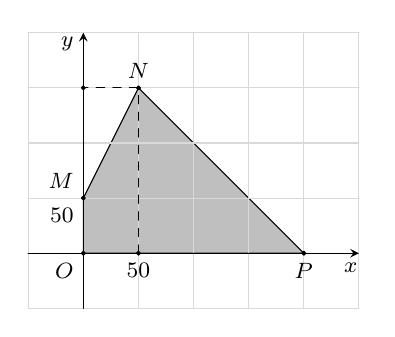
\begin{tikzpicture}[scale=0.7,>=stealth,line join=round,line cap=round,font=\footnotesize]
			\def\xmin{-1} 
			\def\xmax{5}
			\def\ymin{-1} 
			\def\ymax{4} 
			\draw [fill=gray!50] (0,0)--(0,1)--(1,3)--(4,0)--cycle;
			\draw [gray!30] (\xmin,\ymin) grid (\xmax,\ymax);
			\draw [fill=black] (0,0) circle (1pt) node [below left] {$O$}
			(1,0) circle (1pt) node [below] {$50$}
			(0,1) circle (1pt) node [below left] {$50$}
			(0,1) node [above left] {$M$}
			(0,3) circle (1pt)
			(4,0) circle (1pt) node [below] {$P$}
			(1,3) circle (1pt) node [above] {$N$}
			;
			\draw [dashed] (1,0)--(1,3)--(0,3);
			\draw [->] (\xmin,0)--(\xmax,0) node [below, xshift=-3pt] {$x$};
			\draw [->] (0,\ymin)--(0,\ymax) node [left, yshift=-4pt] {$y$};
		\end{tikzpicture}
	}
	\shortans{$-250$}
	\loigiai{
		Giá trị nhỏ nhất của biểu thức $T(x;y)=x-2y$ đạt được tại một trong các đỉnh của tứ giác $OMNP$. \\
		Từ hình vẽ ta có $O(0;0)$, $M(0;50)$, $N(50;150)$ và $P(200;0)$. \\
		Tính giá trị của biểu thức $T(x;y)$ tại các đỉnh $O$, $M$, $N$, $P$ ta được 
		\begin{eqnarray*}
			&&T(0;0)=0-2 \cdot 0=0. \\
			&&T(0;50)=0-2 \cdot 50=-100. \\
			&&T(50;150)=50-2 \cdot 150=-250. \\
			&&T(200;0)=200-2 \cdot 0=200.
		\end{eqnarray*}
		Vậy $T(x;y)$ đạt giá trị nhỏ nhất bằng $-250$. 
	}
\end{ex}
% Câu 2
	\begin{ex}[Trích đề thi dự bị CHKI - Khối 10 - chuyên Lê Quý Đôn Ninh Thuận Năm học 2024 - 2025]%[0D2V2-3]%[Dự án D - đợt 2 NH24-25 - VU Ngoc Hao]
	Một công ty, trong một tháng cần sản xuất ít nhất $12$ viên kim cương to và $9$ viên kim cương nhỏ. Từ 1 tấn Cacbon loại 1 (giá $100$ triệu đồng) có thể chiết xuẩt được $6$ viên kim cương to và $3$ viên kim cương nhỏ, từ 1 tẩn Cacbon loại 2 (giá $40$ triệu đồng) có thể chiết xuất được $2$ viên kim cương to và $2$ viên kim cương nhỏ. Mỗi viên kim cương to có giá $20$ triệu đồng, mỗi viên kim cương nhỏ có giá $10$ triệu đồng. Hỏi trong một tháng công ty này thu về được nhiều nhất là bao nhiêu triệu tiền, biểt rẳng mỗi tháng chỉ có thể sử dụng tối đa $4$ tấn Cacbon mỗi loại?
	\shortans{$280$}
	\loigiai{
		\textbf{Phân tích bài toán:}\\
		Gọi $x$ và $y$ lần lượt là số tấn Cacbon loại 1 và loại 2 mà công ty này sử dụng để chiết xuất kim cương \quad $(x, y \geq 0)$.\\
		Số tiền mua nguyên liệu là: $100 x+40 y$ (triệu đồng).\\
		Với nguyên liệu trên sẽ sản xuất được $6 x+2 y$ viên kim cương to và $3 x+2 y$ viên kim cưong nhỏ.\\
		Số tiền thu được từ các viên kim cương là:
		$(6 x+2 y) \cdot 20+(3 x+2 y) \cdot 10=150 x+60 y$ (triệu đồng).\\
		Lợi nhuận hàng tháng của công ty là:
		$f(x, y)=50 x+20 y$ (triệu đồng). \\
		\textbf{Bài toán trở thành:} Xác định $x,y$ thỏa mãn hệ 	
		\[\left\{\begin{array}{l}6 x+2 y \geq 12 \\ 3 x+2 y \geq 9 \\ 0 \leq x , y \leq 4 \end{array}\right. (*).\]
		\immini{Ta cần tìm giá trị lớn nhất của hàm số $f(x, y)$ trền miền nghiệm của hệ (*).\\
			Miền nghiệm của hệ (*) là ngũ giác (kể cả biên) với các đỉnh $(2/3,4),(1,3),(4,4),(3,0),(4,0)$.\\}{
			\begin{tikzpicture}
				\draw[step=1,gray, very thin,opacity=0.5]
				(-1,-1) grid (5,5);
				\draw [->,blue] (-1,0) -- (5,0) node[above] {$x$};
				\draw [->,blue] (0,-1) -- (0,5) node[right] {$y$};
				\foreach \x in {2/3,1,2,3,4} {\draw (\x /3,0) node[below,blue] {$\x$} circle (1pt);}
				\foreach \y in {3,4,4.5,6} {\draw (0,\y /3) node[left,blue] {$\y$} circle (1pt);}
				\draw (0,0) node [below left]{$O$};
				
				\fill[pattern = north east lines,pattern color = blue!50] plot(-1,-1) -- plot(0,-1) -- plot(0,5) -- plot(-1,5) -- cycle;
				
				\draw[-,blue,thick] (-1,4/3) -- (5,4/3) node[right] {$y=4$};
				\fill[pattern = north east lines,pattern color = blue!50] plot(-1,4/3) -- plot(5,4/3) -- plot(5,5) -- plot(-1,5) -- cycle;
				
				\fill[pattern = north east lines,pattern color = blue!50] plot(-1,-1) -- plot(-1,0) -- plot(5,0) -- plot(5,-1) -- cycle;
				
				\draw[-,blue,thick] (4/3,-1) -- (4/3,5) node[right] {$x=4$};
				\fill[pattern = north west lines,pattern color = blue!50] plot(4/3,-1) -- plot(4/3,5) -- plot(5,5) -- plot(5,-1) -- cycle;
				
				\draw[red,thick,domain=-1:1] plot (\x,{2 - 3*\x}) node[below left] {$6x+2y=12$};
				\fill[pattern = north west lines,pattern color = red!50] plot(-1,-1) -- plot[domain=-1:1](\x,{2 -3*\x}) -- cycle;
				
				\draw[orange,thick,domain=-1:5/3] plot (\x,{3/2 - 3/2*\x}) node[below right] {$3x+2y=9$};
				\fill[pattern = north west lines,pattern color = orange!50] plot(-1,-1) -- plot[domain=-1:5/3](\x,{3/2 -3/2*\x}) -- plot(5/3,-1) -- cycle;
		\end{tikzpicture}}
		\noindent
		Hàm số $f(x;y)$ sẽ đạt giả trị lớn nhất khi $(x, y)$ là toạ độ của một trong các đỉnh $(2/3,4),(1,3),(4,4),(3,0),(4,0)$.\\
		Suy ra: $\max f(x;y)=f(4;4)=280$. Như vậy mỗi tháng công ty này có thể thu về nhiều nhất 280 triệu tiền lãi.	
	}
\end{ex}
\begin{ex}[Trích đề thi chính thức CHKI - Khối 10 - chuyên Lê Quý Đôn Ninh Thuận Năm học 2024 - 2025]%[0D2V2-3]%[Dự án đề kiểm tra Toán khối 10 HK1 NH24-25-Dot2-Nhật Thiện]%[Chuyên Lê Quý Đôn - Ninh Thuận]
	Trong một cuộc thi pha chế đồ uống gồm $2$ loại $A$ và $B$, mỗi đội chơi được sử dụng tối đa $9$ cốc nước lọc, $210$ g đường và $24$ g hương liệu. Để pha chế $1$ cốc đồ uống loại $A$ cần $1$ cốc nước lọc, $30$ g đường, $1$ g hương liệu. Để pha chế $1$ cốc đồ uống loại $B$ cần $1$ cốc nước lọc, $10$ g đường và $4$ g hương liệu. Mỗi cốc đồ uống loại $A$ nhận được $6$ điểm thưởng, mỗi cốc đồ uống loại $B$ nhận được $8$ điểm thưởng. Gọi $x$ là số cốc đồ uống loại $A$ và $y$ số cốc đồ uống loại $B$ cần pha chế. Khi đó số điểm thưởng cao nhất bằng bao nhiêu?
	\shortans{64}
	\loigiai{
		Ta có $x\ge 0$, $y\ge 0$, $x\in \mathbb{N}$, $y\in \mathbb{N}$.\\
		Mỗi đội pha chế được sử dụng tối đa $9$ cốc nước, $210$\,g đường và $24$\,g hương liệu suy ra
		\[\heva{&x+y\le 9\\&30x+10y\le 210\\&x+4y\le 24.}\Leftrightarrow\heva{&x+y\le 9\\&3x+y\le 21\\&x+4y\le 24.}\]
		Ta có miền nghiệm của hệ bất phương trình là miền đa giác $OABCD$ với $O(0;0)$, $A(7;0)$, $B(6;3)$, $C(4;5)$, $D(0;6)$.
		\begin{center}
			\begin{tikzpicture}[scale=1, font=\footnotesize, line join=round, line cap=round, >=stealth]
				\begin{scope}
					\clip (-1,-1) rectangle (10,8);
					\fill[opacity=.2,pattern=north east lines] (0,-1)--(-1,-1)--(-1,8)--(0,8)--cycle;
					\fill[opacity=.2,pattern=north east lines] (-1,0)--(-1,-1)--(10,-1)--(10,0)--cycle;
					\fill[opacity=.2,pattern=north east lines] (-2,11)--(11,11)--(11,-2)--cycle;
					\fill[opacity=.2,pattern=north east lines] (-2,27)--(11,27)--(11,-12)--cycle;
					\fill[opacity=.2,pattern=north east lines](-9,8.25)--(29,8.25)--(29,-1.25)--cycle;
					\draw (1,8)--(10,-1);
					\draw (4.33,8)--(7.33,-1);
					\draw (-8,8)--(28,-1);
					\draw[fill=black] (7,0) circle (1pt) node[above right]{$A$} (6,3) circle (1pt) node[above right]{$B$} (4,5) circle (1pt) node[above right]{$C$} (0,6) circle (1pt) node[above right]{$D$};
				\end{scope}
				\draw[->] (-1,0)--(10,0) node[below]{$x$};
				\draw[->] (0,-1)--(0,8) node[left]{$y$};
				\draw (0,0) node[below left]{$O$};
				\foreach \x/\nx in {1/1,2/2,3/3,4/4,5/5,6/6,7/7,8/8,9/9}
				\draw (\x,1pt)--(\x,-1pt) node[below]{$\nx$};
				\foreach \y/\ny in {1/1,2/2,3/3,4/4,5/5,6/6,7/7}
				\draw (1pt,\y)--(-1pt,\y) node[left]{$\ny$};
				\draw[dashed] (0,5)--(4,5)--(4,0) (0,3)--(6,3)--(6,0);
			\end{tikzpicture}
		\end{center}
		Mỗi cốc đồ uống loại $A$ nhận được $6$ điểm thưởng, mỗi cốc đồ uống loại $B$ nhận được $8$ điểm thưởng. \\
		Gọi $T$ là điểm thưởng, khi đó $T=6x+8y$.\\
		Ta có bảng sau
		\begin{longtable}{|c|c|c|c|c|c|}
			\hline
			& $O(0;0)$ &$A(7;0)$ &$B(6;3)$& $C(4;5)$& $D(0;6)$\\
			\hline
			$T=6x+8y$& $0$& $42$ &$60$ &$64$ &$48$\\
			\hline
		\end{longtable}
		Điểm thưởng cao nhất đạt được bằng $64$ khi $x=4$ và $y=5$.\\
	}
\end{ex}
\Closesolutionfile{ans}

\begin{center}
	\textbf{PHẦN 4 - TỰ LUẬN}
\end{center}
\setcounter{ex}{0}
% Câu 1
\begin{ex}%[0D2V1-3]%[Dự án D - đợt 2 NH24-25 - VU Ngoc Hao]
	Công ty viễn thông Mobifone tính phí $1$ nghìn đồng mỗi phút gọi nội mạng, $2$ nghìn đồng mỗi phút gọi ngoại mạng. Mỗi tháng Minh gọi điện thoại hết từ $200$ đến $300$ nghìn đồng. Viết bất phương trình bậc nhất hai ẩn mô tả cho số tiền điện thoại trả cho ($x$) phút gọi nội mạng và ($y$) phút gọi ngoại mạng trong một tháng.
	\loigiai{
		Số tiền điện thoại trả cho $x$ phút gọi nội mạng là $x$ nghìn đồng.\\
		Số tiền điện thoại trả cho $y$ phút gọi nội mạng là $2y$ nghìn đồng.\\
		Mỗi tháng Minh gọi điện thoại hết từ $200$ đến $300$ nghìn đồng nên ta có 
		\[200\le x+2y\le 300.\]
	}
\end{ex}
% Câu 2
\begin{ex}%[0D2V2-3]%[Dự án D - đợt 2 NH24-25 - VU Ngoc Hao]
	Một công ty cần thuê xe vận chuyển $140$ người và $9$ tấn hàng hóa. Nơi cho thuê xe chỉ có $10$ xe hiệu MITSUBISHI và $9$ xe hiệu FORD. Một chiếc xe hiệu MITSUBISHI có thể chở $20$ người và $0.6$ tấn hàng. Một chiếc xe hiệu FORD có thể chở $10$ người và $1.5$ tấn hàng. Tiền thuê một xe hiệu MITSUBISHI là $4$ triệu đồng, một xe hiệu FORD là $3$ triệu đồng. Hỏi phải thuê bao nhiêu xe mỗi loại để chi phí thấp nhất?
	\dapso{$5$  chiếc MITSUBISHI và $4$ chiếc FORD}
	\loigiai{
		\textbf{Phân tích bài toán:}\\
		Gọi $x$ là số chiếc xe hiệu MITSUBISHI và $y$ là số chiếc xe hiệu FORD công ty cần thuê \quad $(x,y \geq 0)$\\
		Vì nơi thuê xe chỉ có $10$ xe hiệu MITSUBISHI và $9$ xe hiệu FORD nên ta có $0 \leq x \leq 10$ và $0 \leq y \leq 9$.\\
		Theo giả thiết đề bài, ta có thêm điều kiện $20x + 10y \leq 140$ hay $2x + y \leq 14$, $0{,}6x + 1{,}5y \leq 9$.\\
		Tiền thuê xe tổng cộng là $T(x,y) = 4x + 3y$ triệu đồng.\\
		\textbf{Bài toán trở thành:} Xác định $x,y$ thỏa mãn hệ 
		\[\left\{ {\begin{array}{*{20}{c}}
				{0 \leq x \leq 10} \\ 
				{0 \leq y \leq 9} \\ 
				{2x + y \leq 14} \\ 
				{0{,}6x + 1{,}5y \leq 9} 
		\end{array}}\quad(*) \right.\]
		sao cho $T(x,y) = 4x + 3y$ đạt giá trị nhỏ nhất.\\
		Trong mặt phẳng tọa độ vẽ các đường thẳng
		$(d)\colon 2x + y = 14,\left(d^{\prime}\right)\colon 0{,}6x + 1{,}5y = 9,\left(d^{\prime \prime}\right)\colon x=10,\left(d^{\prime \prime \prime}\right)\colon y=9$.\\
		Khi đó miền nghiệm của hệ bất phương trình (*) là phần mặt phẳng(tứ giác) không tô màu trên hình vẽ.
		\begin{center}
			\begin{tikzpicture}
				\draw[step=1,gray, very thin,opacity=0.5]
				(-2,-2) grid (8,8);
				\draw [->,green] (-2,0) -- (8,0) node[above] {$x$};
				\draw [->,blue] (0,-2) -- (0,8) node[right] {$y$};
				\foreach \x in {2.5,5,7,10,15} {\draw (\x /2,0) node[below,blue] {$\x$} circle (1pt);}
				\foreach \y in {2,4,6,9,14} {\draw (0,\y /2) node[left,blue] {$\y$} circle (1pt);}
				\draw (0,0) node [below left]{$O$};
				
				\draw[-,blue,thick] (5,-2) -- (5,8) node[right] {$x=10$};
				\fill[pattern = north east lines,pattern color = blue!50] plot(5,-2) -- plot(5,8) -- plot(8,8) -- plot(8,-2) -- cycle;
				
				\fill[pattern = north east lines,pattern color = blue!50] plot(-2,-2) -- plot(0,-2) -- plot(0,8) -- plot(-2,8) -- cycle;
				
				\draw[-,green,thick] (-2,4.5) -- (8,4.5) node[right] {$y=9$};
				\fill[pattern = north west lines,pattern color = green!50] plot(-2,4.5) -- plot(8,4.5) -- plot(8,8) -- plot(-2,8) -- cycle;
				
				\fill[pattern = north east lines,pattern color = green!50] plot(-2,-2) -- plot(-2,-0) -- plot(8,0) -- plot(8,-2) -- cycle;
				
				\draw[red,thick,domain=-0.5:4.5] plot (\x,{7 - 2*\x}) node[right] {$2x+y=14$};
				\fill[pattern = north west lines,pattern color = red!50] plot(-2,-2) -- plot(-2,8) -- plot(-0.5,8) --  plot[domain=-0.5:4.5](\x,{7 -2*\x}) -- plot(4.5,-2) -- cycle;
				
				\draw[orange,thick,domain=-2:8] plot (\x,{3 - 0.4*\x}) node[right] {$0.6x+1.5y=9$};
				\fill[pattern = north west lines,pattern color = orange!50] plot(-2,-2) -- plot[domain=-2:8](\x,{3 - 0.4*\x}) -- plot(8,-2) -- cycle;
			\end{tikzpicture}
		\end{center}
		Giá trị nhỏ nhất của $T(x,y) = 4x + 3y$ đạt tại một trong các điểm $(2.5;9),(5;4),(10;2), (10;9)$.\\
		Ta có\\
		$T(2.5;9)= 4 \cdot 2.5 + 3 \cdot 9 = 37$.\\
		$T(5;4)= 4 \cdot 5 + 3 \cdot 4 = 32$.\\
		$T(10;2)= 4 \cdot 10 + 3 \cdot 2 = 46$.\\
		$T(10;9)= 4 \cdot 10 + 3 \cdot 9 = 67$.\\
		suy ra giá trị nhỏ nhất của $T(x;y)$ là $32$ khi $(x;y)=(5;4)$.\\
		Vậy công ty phải thuê $5$  chiếc MITSUBISHI và $4$ chiếc FORD để chi phí thấp nhất.
	}
\end{ex}
% Câu 3
	\begin{ex}%[0D2V2-3]%[Dự án D - đợt 2 NH24-25 - VU Ngoc Hao]
	Một cơ sở sản xuất dự định sản xuất ra hai loại sản phầm $A$ và $B$. Các sản phẩm này được chế tạo ra từ ba loại nguyên liệu I, II và III. Số lượng đơn vị dự trữ của từng loại nguyên liệu và số lượng đơn vị từng loại nguyên liệu cần để sàn xuất ra một đơn vị sản phầm mỗi loại được cho tương ứng trong bảng sau:
	\begin{center}
		\scalebox{0.9}{
			\begin{tabular}{|c|c|c|c|}
				\hline \multirow{2}{*}{ Loại nguyên liệu } & \multirow{2}{*}{ Nguyên liệu dự trữ mỗi tuần } & \multicolumn{2}{|c|}{ Số đơn vị cần dùng cho một đơn vị sản phẩm } \\
				\cline { 3 - 4 } & & Sản phẩm $A$ & Sản phẩm $B$ \\
				\hline I & 18 & 2 & 3 \\
				\hline II & 30 & 5 & 4 \\
				\hline III & 25 & 1 & 6 \\
				\hline
		\end{tabular}}
	\end{center}
	\noindent
	Mỗi đơn vị sản phẩm $A$ lãi $300000$ đồng, mỗi đơn vị sản phẩm $B$ lãi $200000$ đồng. Hãy cho biết với kế hoạch sản xuất như thế nào thì số tiền lãi thu được hàng tuần là lớn nhất.
	\dapso{$33$ sản phẩm $A$ và $32$ sản phẩm $B$}
	\loigiai{
		\textbf{Phân tích bài toán:}\\
		Gọi $x$ và $y$ lần lượt là số sản phẩm $A$ và $B$ mà đơn vị này sản xuất hàng tuần \quad $(x, y \geq 0)$.\\
		Lợi nhuận thu được hàng tuần là:\\
		$$f(x;y)=300000 x+200000 y \text { (đồng). }$$ \\
		Theo giả thiết đề bài, ta có thêm điều kiện \[\left\{\begin{array}{l}
			2 x+3 y \leq 18 \\
			5 x+4 y \leq 30 \\
			x+6 y \leq 25 \\
			x;y \geq 0.
		\end{array}\right. \text { (*) }\]
		\textbf{Bài toán trở thành:} Tìm giá trị lớn nhất của hàm số $f(x, y)$ trên miền nghiệm của hệ bất phương trình $(*)$.\\
		Miền nghiệm của hệ bất phương trình (*) là tứ giác không tô màu (kể cả biên).\\
		\begin{center}
			\begin{tikzpicture}
				\draw[step=1,gray, very thin,opacity=0.5]
				(-2,-2) grid (7,7);
				\draw [->,blue] (-2,0) -- (7,0) node[above] {$x$};
				\draw [->,blue] (0,-2) -- (0,7) node[right] {$y$};
				\foreach \x in {6,9,25} {\draw (\x /5,0) node[below,blue] {$\x$} circle (1pt);}
				\foreach \y in {6,25/6,15/2} {\draw (0,\y /5) node[left,blue] {$\y$} circle (1pt);}
				\draw (0,0) node [below left]{$O$};
				
				\fill[pattern = north east lines,pattern color = blue!50] plot(-2,-2) -- plot(-2,0) -- plot(7,0) -- plot(7,-2) -- cycle;
				
				\fill[pattern = north west lines,pattern color = blue!50] plot(-2,-2) -- plot(0,-2) -- plot(0,7) -- plot(-2,7) -- cycle;
				
				\draw[red,thick,domain=-2:4.8] plot (\x,{6/5 - 2/3*\x}) node[below right] {$2x+3y=18$};
				\fill[pattern = north west lines,pattern color = red!50] plot(7,7) -- plot(-2,7) -- plot[domain=-2:4.8](\x,{6/5 -2/3*\x}) -- plot(7,-2) -- cycle;
				
				\draw[orange,thick,domain=-2:2.8] plot (\x,{3/2 - 5/4*\x}) node[below left] {$5x+4y=30$};
				\fill[pattern = north east lines,pattern color = orange!50] plot(7,7) -- plot(-2,7) -- plot[domain=-2:2.8](\x,{3/2 -5/4*\x}) -- plot(7,-2) -- cycle;
				
				\draw[green,thick,domain=-2:7] plot (\x,{5/6 - 1/6*\x}) node[below right] {$5x+4y=30$};
				\fill[pattern = north east lines,pattern color = green!50] plot(7,7) -- plot(-2,7) -- plot[domain=-2:7](\x,{5/6 -1/6*\x}) -- plot(7,-2) -- cycle;
			\end{tikzpicture}	
		\end{center}
		\noindent
		Hàm số $f(x;y)$ sẽ đạt giá trị lớn nhất khi $(x;y)$ là toạ độ của một trong các đỉnh $(0;0)$, $(6;0)$, $\left(\dfrac{11}{3};\dfrac{32}{9}\right)$, $\left(0;\dfrac{25}{6}\right)$. \\
		Ta có: $f(0;0)=0$, $f(6;0)=1\,800\,000$, $f\left(\dfrac{11}{3};\dfrac{32}{9}\right)=\dfrac{16300000}{9}, f\left(0;\dfrac{25}{6}\right)=\dfrac{2500000}{3}$. \\
		Suy ra $f(x, y)$ lớn nhất khi $(x, y)=\left(\dfrac{11}{3};\dfrac{32}{9}\right)$ tức là xưởng này cần sản xuất $33$ sản phẩm $A$ và $32$ sản phẩm $B$ trong vòng $9$ tuần để thu lợi nhuận cao nhất.
	}
\end{ex}
